\subsection{Introducción:}

En este ejercicio vamos a realizar la Tabla de Descriptores Globales (\textit{GDT}). Se pide que realizemos lo siguiente :

\begin{itemize}
\item [\textit{a)}] Que la tabla \textit{GDT} tenga 4 segmentos, dos para código de
nivel 0 y 3; y otros dos para datos de nivel 0 y 3. Estos segmentos deben direccionar los primeros 500MB de memoria. Por último se pide no usar las primeras siete posiciones de la \textit{GDT}, ya que se consideran utilizadas.

\item [\textit{b)}] Pasar a modo protegido y setear la pila del kernel en la dirección 0x27000. 

\item [\textit{c)}] Agregar a la \textit{GDT} un segmento adicional y escribir una rutina qe utilice este nuevo segmento para pintar la esquina superior izquierda de la pantalla.

\item [\textit{d)}] Limpiar la pantalla y pintar el área del mapa (sugerido el color gris) junto con las barras inferiores para los jugadores.
\end{itemize}

\subsection{Ítem a): Setear la \textit{GDT}}

Para este ítem completamos el archivo \textit{GDT}.c proporcionado por la catedra. En el mismo la \textit{GDT} es representada mediante un array de 30 posiciones. Cada posicion tiene la siguiente estructura.
\\

\begin{figure}[H]
\begin{center}
\minipage{0.6\textwidth}
  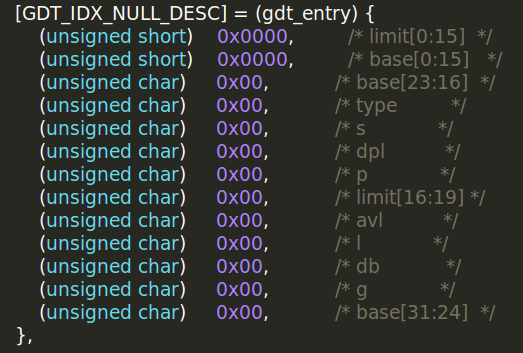
\includegraphics[width=\linewidth]{ejercicio1/GDTnula.png}
  \caption{{\small Este descriptor corresponde a la primer entrada de la \textit{GDT}}} 
\endminipage
\end{center}
\end{figure}

Como la primer posicion de la tabla \textit{GDT} debe ser corresponder a una entrada nula, llenamos la primer posicion como muestra la imagen debajo.
\\


Luego, creamos los 4 segmentos que se piden a partir de la posicion 8 de la \textit{GDT}, ya que por enunciado, no se deben tocar las primeras 7 posiciones de la table de descriptores. Mostramos en las imagenes de abajo como creamos un descriptor de datos y otro de codigos. 
\\

\begin{figure}[H]
\begin{center}
\minipage{0.5\textwidth}
  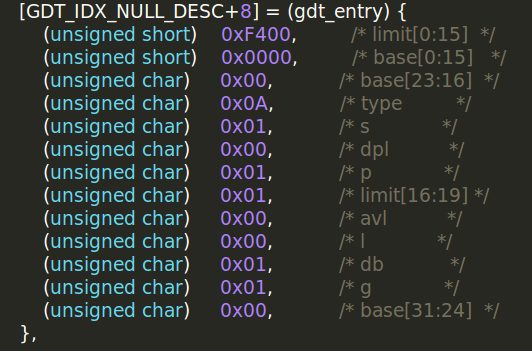
\includegraphics[width=\linewidth]{ejercicio1/GDTcodigo0.png}
  \caption{{\small Este descriptor corresponde al segmento de datos de nivel 0}} 
\endminipage
\minipage{0.5\textwidth}
  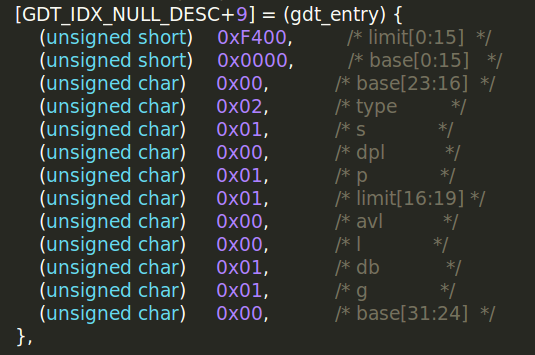
\includegraphics[width=\linewidth]{ejercicio1/GDTdatos0.png}
  \caption{{\small Este descriptor corresponde al segmento de código de nivel 0}} 
\endminipage
\end{center}
\end{figure}

Los otros dos que faltan son exactamente iguales, solo que en la linea correspondiente al nivel (dpl) ponemos 0x03, ya que corresponde al nivel 3 de prioridad.\\

Los descriptores de segmentos tienen la siguiente forma:
\\

\begin{figure}[H]
\begin{center}
\minipage{0.8\textwidth}
  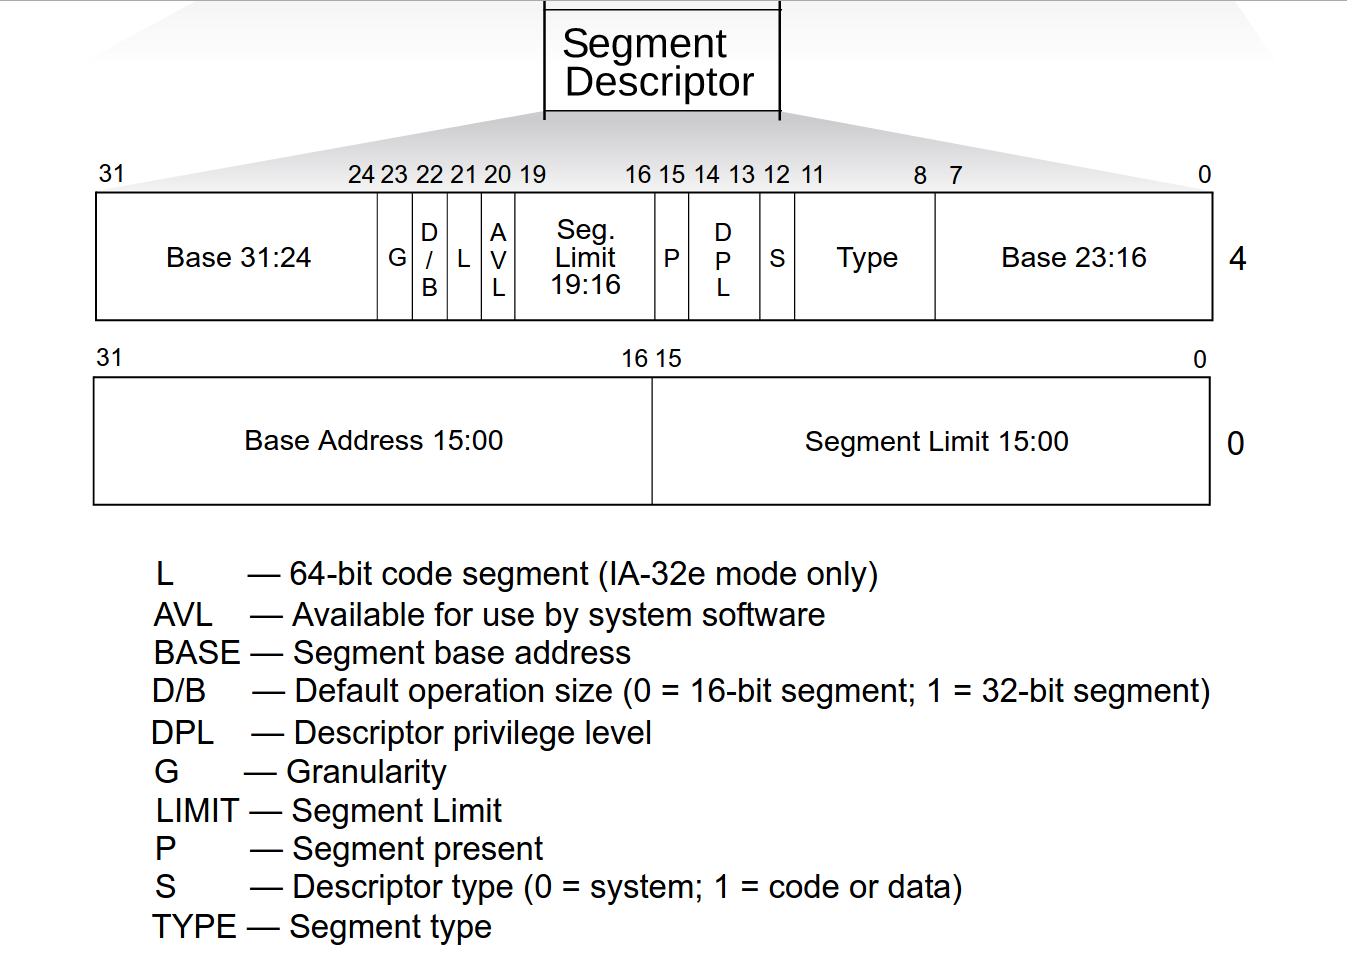
\includegraphics[width=\linewidth]{ejercicio1/estructuradescriptor.png}
  \caption{{\small Este descriptor corresponde a la primer entrada de la \textit{GDT}}} 
\endminipage
\end{center}
\end{figure}

Completamos nuestros descriptores como marcan las figuras 3 y 4 de esa forma porque:

\begin{itemize}
\item [\textit{Base:}] En el tp se pide que los descriptores direcciones los primeros 500mb de memoria. Por ende la base corresponde a la dirección 0x00000000.
\item [\textit{G:}]  Para poder direccionar 500mb, no nos alcanza la cantidad de bits que hay para el limite, por ende necesitamos activar la granularidad para poder abarcar más memoria, ya que cuando esta activada la posicion que indica el limite se multiplica por 4kb.
\item [\textit{Límite:}] Como esta activada la granularidad, podemos abarcar 500mb de memoria, el limite correspondiente a 500mb con la granularidad activada es 0x0F400.
\item [\textit{Type:}] Aqui se indica si el descriptor es de código/datos, a los correspondientes a datos les pusimos que eran de tipo 0x02 (segmento de datos de escritura/lectura) y a los de código que eran de tipo 0x0A (segmentdo de código de escritura/lectura).
\item [\textit{S:}] Con este bit se decide si es un segmento de sistema (s=0) o si son de código/data (s=1), por ende a este bit le corresponde un 0x1.
\item [\textit{Dpl:}] En esta seccion se declara el privilegio del segmento, a los que eran de nivel 0 les corresponde un 0x00 y a los de nivel 3 un 0x03
\item [\textit{P:}] Este es el bit de present. Cuando es ’1’ el segmento correspondiente esta presente en la memoria RAM. Si es ’0’, el segmento esta en la memoria virtual. Por ende lo seteamos en 1.
\item [\textit{Avl:}] Es el bit correspondiente a Available. Como no lo vamos a tener en cuenta lo dejamos en 0.
\item [\textit{L:}] Indica si el código es de 64bits o de 32. Como trabajamos en 32bits dejamos este bit en 0.
\item [\textit{D/B:}] Este bit define el tamaño de las operaciones en las que va a trabajar el procesador. De nuevo, como nos encontramos trabajando en 32bits, el tamaño de las operaciones debe ser de 32, por eso lo seteamos en 1.
\end{itemize}

\subsection{Ítem b): Pasar a modo protegido y setear la pila}

Para pasar a modo protegido realizamos los siguientes pasos:

\begin{itemize}
\item [\textit{a)}] Deshabilitamos las interrupciones, para eso utilizamos la instrucción CLI.

\item [\textit{b)}] Cargamos el registro \textit{GDTR} con la dirección base de la \textit{\textit{GDT}} utilizando la instrucción \textit{LGDT} de esta manera: 
\begin{center}
lgdt [GDT DESC]
\end{center}
Donde GDT DESC es el descriptor de la tabla.

 \item [\textit{c)}] Seteamos el bit \textit{PE} (BIT 0) del registro \textit{CR0} en 1 para pasar a modo protegido. Procedemos a hacer esto con las intrucciones:
\begin{center}
      mov eax, cr0\\
     or eax, 1   $~~~~$ \\
       mov cr0, eax
    \end{center}

\item [\textit{d)}]Realizamos un far jump para cargar en el registro \textit{CS} la dirección donde esta el segmento de código. Para esto utilizamos la instruccion: 

\begin{center}
jmp 0X40:modoprotegido
\end{center}

Donde 0x40 es la dirección donde en nuestra \textit{GDT} compienza el segmento de código y modoprotegido es una etiqueta que se encuentra imediatamente debajo de este JMP. 

\item [\textit{e)}]Cargamos los registros de segmento de la siguiente manera.

\begin{center}
   mov ax, 0x48\\
    mov ds, ax$~~~$\\
    mov ax, 0x48\\
    mov ss, ax$~~~$\\
\end{center}


\end{itemize}

Ahora que ya nos encontramos con el procesador trabajando en modo protegido, procedemos a setear la pila en la dirección 0x27000. Para eso seteamos los registros ebp y esp en la dirección 0x27000 con las siguientes instrucciones: 
\begin{center}
mov ebp, 0x27000\\
mov esp, 0x27000\\
\end{center}

\subsection{Ítem c): Agregar a la \textit{GDT}  un segmento adicional y utilizarlo como memoria de vídeo}

Para este ítem, agregamos a la \textit{GDT} el siguiente segmento, el cual direcciona a la memoria de vídeo utilizada por la pantalla (Desde 0xB8000 a 0XC000).

\begin{figure}[H]
\begin{center}
\minipage{0.5\textwidth}
  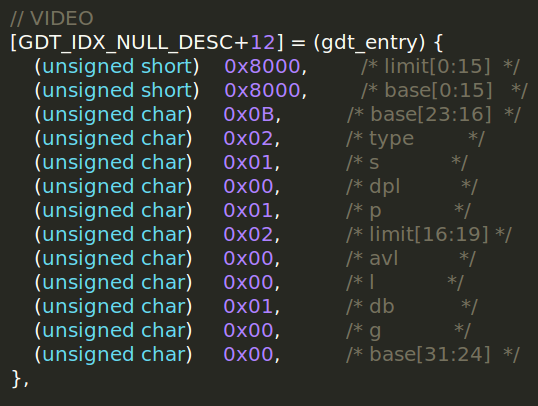
\includegraphics[width=\linewidth]{ejercicio1/memvid.png}
  \caption{{\small}} 
\endminipage
\end{center}
\end{figure}


Luego cargamos en un registro de segmento, en este caso  \textit{FS}, la posicion del segmento anterior. Por ultimo con las siguiente instrucción podemos poner en la esquina superior izquierda de la pantalla lo que querramos
\begin{center}
mov word[fs:0x00],  \textit{aimprimir}
\end{center}

Donde  \textit{aimprimir} es algo de tamaño word, y su valor es el que aparece en la esquina superior izquierda de la pantalla. Esto ocurre porque se carga el segmento que comienza en la dirección a que la dirección 0xB8000 y se le suma el offset 0 y esta es la primer dirección de la memoria de vídeo utilizada por la pantalla.\\

Si por ejemplo escribimos la siguiente línea:
\begin{center}
mov word[fs:0x00],  0xdb00
\end{center}

Obtenemos este resultado, que es lo que pedía el ejercicio.

\begin{figure}[H]
\begin{center}
\minipage{0.8\textwidth}
  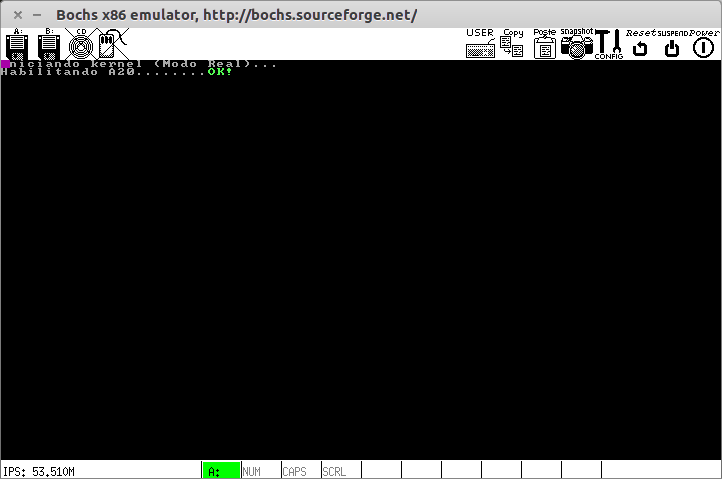
\includegraphics[width=\linewidth]{ejercicio1/esqsupizq.png}
  \caption{{\small}} 
\endminipage
\end{center}
\end{figure}

\subsection{Ítem d): Limpiar la pantalla y pintar el área del mapa}

En este punto creamos una función auxiliar en C para limpiar la pantalla. La función pinta la pantalla de gris y es la siguiente:

\begin{figure}[H]
\begin{center}
\minipage{0.3\textwidth}
  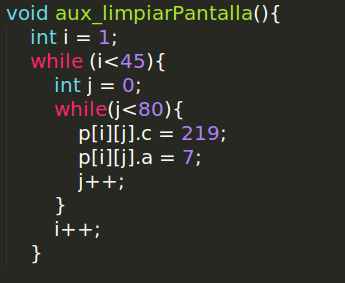
\includegraphics[width=\linewidth]{ejercicio1/limpant.png}
  \caption{{\small}} 
\endminipage
\end{center}
\end{figure}

Esta función la escribimos en \textit{screen.c} y utiliza la matriz P creada por la catedra para acceder a las posiciones de la pantalla. Estos son los resultados luego de utilizar nuestra función. \\

\begin{figure}[H]
\begin{center}
\minipage{0.8\textwidth}
  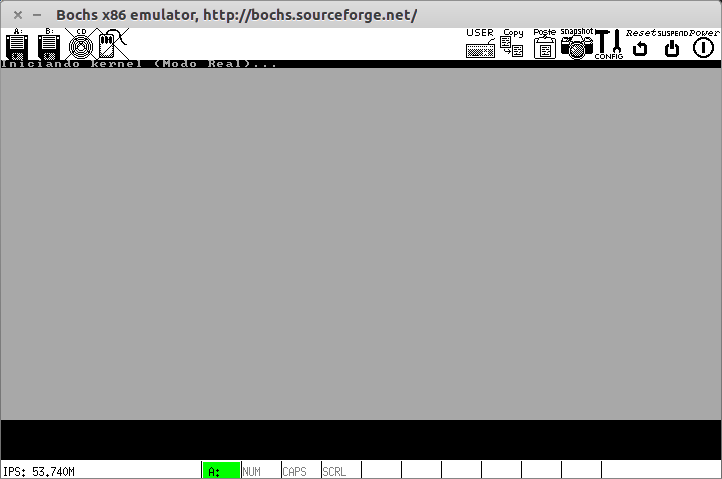
\includegraphics[width=\linewidth]{ejercicio1/pantgris.png}
  \caption{{\small}} 
\endminipage
\end{center}
\end{figure}


Para pintar el mapa utilizamos la función dada por la catedra  \textit{screen$\_$inicializar}. Para utilizar estas funciones, escribimos en \textit{kernel.asm} las siguientes lineas con el siguiente resultado:

\begin{center}
 call aux$\_$limpiarPantalla    \\
 call screen$\_$inicializar$~~~$
\end{center}

\begin{figure}[H]
\begin{center}
\minipage{0.8\textwidth}
  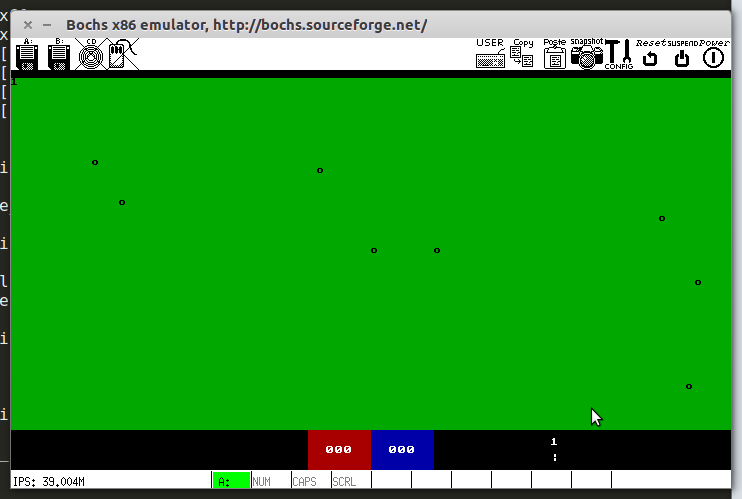
\includegraphics[width=\linewidth]{ejercicio1/mapa.png}
  \caption{{\small}} 
\endminipage
\end{center}
\end{figure}
